\section{Partner-specific linguistic behavior}

\subsection{Priming}

\subsection{Adaptation}



\subsection{Accommodation}


\section{Computational models of adaptation}

\subsection{Phonetic adaptation} ideal adaptor framework

\subsection{Syntactic adaptation} 

Kleinschmidt et al. (2012); 
van Schijndel and Linzen (2018); 

priming models?

\subsection{Prosodic adaptation} Roettger \& Franke

\subsection{Conceptual pacts} Hawkins et al.




\section{The semantics of uncertainty expressions}

While this is not a dissertation about modality, many of the utterances that I consider in my experiments contain an epistemic modal.
Since I discuss the implications of my experimental results for popular theories of the semantic of epistemic modals in Section~{XXX}, and since 
my computational model is inspired by recent accounts of epistemic modality, I provide a brief introduction to several theories of modality in this section.

Here, and throughout this dissertation, I adapt the broad notion of modality by \cite{Portner2009} and \cite{Kratzer2012Ch2}, which not only 
includes modal auxiliaries (e.g., \textit{might}, \textit{could}) but also other evidential devices such as probability operators 
(e.g., \textit{probably}) and attitude verbs (e.g., \textit{think}). At the same time, however, to limit the scope of this discussion,  
I will only cover epistemic modality, and therefore omit any discussion of deontic modals, i.e., modals to express how the 
world should be according to laws, societal norms, etc., which are frequently discussed together with epistemic modals.
I will also omit discussions of the important connections between modals and conditionals \cite{see e.g., Lewis1973?,Kratzer1978,Kratzer1979,Kratzer2012}
and discussions of the extent to which different semantic theories validate desired and undesired logical inferences \cite{see e.g., Yalcin2010}.

\subsection{Background: Possible world semantics}

Classical modal logic and most other semantic theories of modals are based on the concept of possible worlds \cite{kripke1963}.
A possible world is a world which differs in one or multiple properties from the actual world. For example, while the proposition $\phi_{brown}$
expressed by the  sentence ``I have brown hair'' is true in the actual world $w$, one possible world $w_1$ is identical in every regard to 
the actual world except that the proposition $\phi_{blond}$ encoded by ``I have blond hair'' is true and the one encoded by
``I have brown hair'' ($\phi_{brown}$) is false. 

According to  a possible world semantics, all sentences have to be evaluated relative to a possible world $w$ and
propositions $\phi$ can be represented as a set of worlds in which $\phi$ is true. If we consider the worlds $w$ and $w_1$ as described here,
the propositions expressed by the sentences ``I have brown hair'' and ``I have blond hair'' evaluate to different truth conditions, depending on the possible world.

$$\sem{\phi_{brown}}^w = 1 \mbox{ iff } w \in \phi_{brown}  = 1$$
$$\sem{\phi_{brown}}^{w_1} = 1 \mbox{ iff } w_1 \in \phi_{brown}  = 0$$
$$\sem{\phi_{blond}}^{w} = 1\mbox{ iff } w \in \phi_{blond} = 0$$
$$\sem{\phi_{blond}}^{w_1} = 1 \mbox{ iff } w_1 \in \phi_{blond} = 1$$




%* start off with why i'm talking about modals

%* what are modals

%* what are the questions relevant to modality

%* which ones of these are relevant for this thesis

%* Possible worlds

%* Modal logic

%* Kratzer

%* threshold semantics proposals

%* wallsten/budesco




%The semantics of epistemic modals\footnote{I adapt the broad notion of modality by \cite{Portner2009} and \cite{Kratzer2012}, which not only 
%includes modal auxiliaries (e.g., \textit{might}, \textit{could}) but also other evidential devices such as probability operators 
%(e.g., \textit{probably}) and attitude verbs (e.g., \textit{think}).} such as \textit{might}, \textit{could} and \textit{probably} 
%has been extensively discussed in the formal semantics literature. However, a lot of these works focus on how 
%different meaning representation affect logical inferences and how they can be used to compositionally derive the 
%meaning of sentences with modal expressions, which are less relevant debates for the enterprise in this dissertation.
%I therefore primarily give an overview of different formalisms along with a discussion about what they predict
%about the interpretation of epistemic modals when they are used to communicate probabilities of future events.

\subsection{Modal logic}

In classical modal logic, the truth conditions of sentences with epistemic modals depend on an accessibility relation $R$.
$R$ determines which worlds $w'$ are epistemically accessible from the actual world $w$, i.e., which worlds are epistemically consistent with
the actual world. For example, consider rolling two six-sided dice, one after another. Before you roll the first die, all worlds in which the sum of
the two dice is between 2 and 12 (all possible combinations of two dice) are epistemically accessible since they are compatible with the actual
world. Now, if you roll one of the dice and it comes up 4, only worlds in which the sum of the two dice is between 5 and 10 (all possible sums of 4 and 
a number between 1 and 6) are epistemically accessible. 

Formally, if $wRw'$ is true then $w'$ is epistemically accessible from $w$. A proposition $\phi$ embedded under an epistemic modal is then true
if either $\phi$ is  true in all epistemically accessible worlds (for necessity modals such as \textit{must}) or $\phi$ is true in at least one epistemically 
accessible world (for possibility modals such as \textit{might}).

\begin{exe}
\ex \label{ex:modall-must} $\sem{\mbox{must } \phi}^{w}  = 1 \mbox{ iff } \forall w' \in W: wRw' \rightarrow  \sem{\phi}^{w'} = 1$
\ex \label{ex:modall-might} $\sem{\mbox{might } \phi}^{w}  = 1 \mbox{ iff } \exists w' \in W: wRw' \rightarrow  \sem{\phi}^{w'} = 1$
\end{exe}

If we again use the example of rolling two dice and assume that the world $w_x$ corresponds to the sum 
of the two dice being $x$, then $wRw'$ is true iff $w' \in \{w_2, w_3, ..., w_{11}, w_{12}\}$. Therefore, for example,
\begin{align*}
\sem{&\mbox{must roll a number between 2 and 12}}^{w} =  1 \\
 & \mbox{(since \textit{roll a number between 2 and 12} is true in all epistemically accessible worlds)} \\ \\ 
 \sem{&\mbox{must roll a 7}}^{w} =  0 \\
 & \qquad \qquad \qquad \quad \mbox{ (since \textit{roll a 7} is only true in some epistemically accessible worlds)} \\ \\
 \sem{&\mbox{might roll a 7}}^{w} =  1 \\
 &  \qquad \qquad \qquad \qquad \quad \mbox{ (since \textit{roll a 7} is true in the epistemically accessible world }w_7\mbox{)}\\ \\ 
 \sem{&\mbox{might roll a 1}}^{w} =  0 \\
 &  \qquad \qquad \qquad \qquad \qquad \mbox{\  (since \textit{roll a 1} is false in all epistemically accessible worlds).}
\end{align*}

While this approach seems intuitively correct for scenarios like rolling two dice, it is very challenging to represent utterances
that convey more fine-grained meanings than mere possibility or necessity. As \cite{Lassiter2017} points out, one could extend this proposal
to modal expressions such as \textit{probably} and \textit{likely} by assuming that \textit{probably $\phi$} is true if $\phi$ is true in more 
epistemically accessible worlds than epistemically accessible worlds in which $\phi$ is false:
\begin{exe}
\ex $\sem{\mbox{probably} \phi}^{w}  = 1 $ \\ 
 \ \ \ \ \ \ \ \ $ \mbox{ iff } |\{w' \in W \mid wRw' = 1 \land \sem{\phi}^{w'} = 1\}| > |\{w' \in W \mid wRw' = 1 \land \sem{\phi}^{w'} = 0\}|$
\end{exe}
However, this proposal comes with at least two shortcomings if one wants to consider it as a 
complete theory of epistemic modals. First, one has to make the limit assumption \cite{Lewis1981}, i.e., 
one has to assume that $W$ contains a finite number of possible worlds. Second, this proposal does not provide 
a theory of interpretation for any type of graded epistemic modal expressions such as \textit{It is 60\% likely that...} or \textit{It is highly probable that...}
or modal expressions in comparative constructions such as \textit{It is twice as likely that X than Y} \cite{Lassiter2017}. Third, there
is no connection between event probabilities and the use of different modals except that this account would predict that \textit{might $\phi$} is true
when the probability of $\phi$ is greater than 0, and \textit{must $\phi$} is true if the probability of $\phi$ is 1.

%For my experiments, neither of this will be necessarily an issue; I am not dealing with graded expression 
%and the number of future events and hence also the number of possible world is limited. 
%However, two additional issues arise. First, given the previously established inter-subject variability in the interpretation 
%of epistemic modals \cite{Wallsten1986}, we need a theory that can accommodate variability. The only possibility to represent
%variability in this formalism would be to assume that either different speakers use different accessibility relations or different speakers
%use different sets of possible worlds. However, it seems unlikely that speakers who have access to the same kind of information 
%(the same visual stimuli both in \cite{Wallsten1986} and in my experiments) would rely on different accessibility relations or a different set of 
%possible worlds.

%Second, while intuitively this definition of \textit{probably} such that $\sem{\mbox{probably} \phi}^w$ is true if $\phi$ is more likely than $\lnot \phi$ 
%appears to be reasonable, there does not seem to be a similar definition for other uncertainty expression such as \textit{think} or \textit{looks like}.
%We could again assume that there are different accessibility relations associated with 

% and unless we assume
%variable accessibility relations $R$ or variable sets of possible worlds, this theory cannot represent 

% it remains unclear how this theory could predict any type of variability. Second, 



%probably $ wRw' and true / wRw' > 0.5$ 
%might $ wRw' and true / wRw' > 0$ 
%must $ wRw' and true / wRw' = 1$
%very likely $ wRw' and true / wRw' > 0.5 + \theta$
%more likely than $ wRw' and A is true / wRw' > wRw' and B is true / wRw'$

%issues: one has to be very careful how to set up the world structure --> otherwise law of probability no longer holds

%needs again limit assumption

%how is this better from just using probabilities?

\subsection{Double relativity of modals}

The most prominent semantic theory of epistemic modals (and all other flavors of modals) is the account by Kratzer 
\cite{Kratzer1981,1991}, later revised in \cite{Kratzer2012}. Building on \cite{Lewis1973}, she developed a unifying 
account of all modal flavors, which assumes that there are several core meanings of modals that can be expressed 
by various linguistic devices (e.g., \textit{could} and \textit{might} are both possibility modals), and that the interpretation
of a sentence with a modal depends on two \textit{conversational backgrounds}, that is, contextually specified functions 
from possible worlds to sets of propositions: 
the \textit{modal base} $f(w)$ and the \textit{ordering source} $g(w)$. 

The intuition behind the modal base $f(w)$ is that one can explicitly state which worlds the modal quantifies over using an 
``In the view of ...'' adverbial clause. For example, for epistemic modals, the modal base may be a function that returns the set of propositions
that are compatible with what is knowns in the current world, which can be explicitly expressed in a sentence with an epistemic modal through the
adverbial clause ``In the view of what is known'':

\begin{exe}
\ex In the view of what is known, it could rain tomorrow.
\end{exe}

\noindent Kratzer argues that utterances without explicit mention of a conversational background are interpreted
by contextually resolving the relevant modal base. If we ignore the ordering source for a second, this leads to the following 
definitions of $f$-necessity and $f$-possibility.

\begin{quote}
\noindent $f$-\textit{necessity}: \\
$\phi$ is a necessity with respect to a modal base $f$ iff $\phi \subseteq \cap f(w)$.

\noindent $f$-\textit{possibility}: \\
$\phi$ is a possibility with respect to a modal base $f$ iff $\cap \{\{\phi\} \cup  f(w) \} \ne \emptyset$.
\end{quote}

The semantics of sentences with necessity modals such as \textit{must} and possibility modals such as \textit{might}
can then be expressed in terms of $f$-necessity and -possibility:

\begin{exe}
\ex $\sem{\mbox{must }\phi}^{w,f} = 1 \mbox{ iff $\phi$ is an $f$-necessity in $w$} $
\ex $\sem{\mbox{might } \phi}^{w,f} = 1 \mbox{ iff $\phi$ is an $f$-possibility in $w$} $
\end{exe}

The semantics of these expressions is equivalent to the classical modal logic semantics presented in (\ref{ex:modall-must})  and (\ref{ex:modall-might}), 
since the accessibility relation $R$ can be defined as $wRw' = w' \in \cap f(w)$. For this reason, this account suffers from the same
issues as the classical modal logic account: it cannot be used to derive interpretations for graded modals or comparatives.

Kratzer partially resolves these issues by introducing a second conversational background, 
the ordering source $g(w)$. $g(w)$ defines a partial preorder $\le_{g(w)}$ over the set of possible worlds $W$ such that 
$$u \le_{g(w)} v \mbox{ iff } \{ p \in g(w) \mid u \in p \} \subseteq \{ p \in g(w) \mid v \in p \}.$$
That means, $v$ is at least as close to an ideal as $u$ iff all propositions in the set of ideal 
propositions $g(w)$ that are true in $u$ are also true in $v$. In the case of epistemic modals, 
the ideal as defined by $g(w)$, is usually assumed to contain propositions corresponding to a normal course of events.

Necessity and possibility then be defined as follows.
\begin{quote}
\noindent \textit{Necessity}: \\
$\phi$ is a necessity with respect to a modal base $f$ and an ordering source $g$ iff for all $u \in \cap f(w)$, there is a $v \in \cap f(w)$
such that $u \ge_{g(w)} v$ and for all $z \in \cap f(w):$ if $v \ge_{g(w)} z$, then $z \in \phi$.

\noindent \textit{Possibility}: \\
$\phi$ is a possibility with respect to a modal base $f$ and an ordering source $g$ iff $\lnot \phi$ is not a necessity with respect to $f$ and $g$.
\end{quote}
\noindent Intuitively, the definition of necessity can be seen as further restricting the modal source such that something must be true if it is true in 
all epistemically accessible worlds that come closest to the ideal defined by the ordering source. 

To illustrate how the modal base and the ordering source work together, imagine a murder case in a small town in which 
there are four suspects A, B, C, and D who all have a motive.\footnote{Example adapted from \cite{Kratzer2012Ch2}.} Further,
there was a tourist T from Iceland in town when the murder happened. Since random tourists rarely murder somebody without
a motive, the set of normal propositions $g(w)$ in this example could be $\{a, b, c, d\}$, where each proposition corresponds to
 A, B, C, and D committing the murder, respectively. 
However, the conversational background of what is known $f(w)$ is compatible with A, B, C, D, or T being the murderer,
i.e., $\cap f(w) = \cup \{a, b, c, d, t\}$. Now, it seems natural for a police officer to utter (\ref{ex:kratzer-a-murder-might})
or  (\ref{ex:kratzer-abcd-murder-must}) but unlikely for the officer to utter (\ref{ex:kratzer-t-murder-might}).

\begin{exe}
\ex \label{ex:kratzer-a-murder-might} A might have committed the murder.
\ex \label{ex:kratzer-abcd-murder-must} A or B or C or D must have committed the murder.
\ex \label{ex:kratzer-t-murder-might} T might have committed the murder.
\end{exe}

\noindent Kratzer's account makes exactly these predictions. It predicts that (\ref{ex:kratzer-a-murder-might}) is true because 
$\lnot a$ is not a necessity and therefore $a$ is a possbility; it predicts that (\ref{ex:kratzer-abcd-murder-must}) since 
$a \lor b \lor c \lor d$ is a necessity; and it  predicts that (\ref{ex:kratzer-t-murder-might}) is false since $\lnot t = a \lor b \lor c \lor d$ is a necessity
and therefore $t$ is not a possibility.

Apart from introducing this distinction between normal courses of events and theoretically possible courses of events, Kratzer's account also
provides a semantics for comparatives using the notion of comparative possibility.\footnote{This is the revised definition of comparative possibility from
in \cite{Kratzer2012Ch2} which is slightly different from the original notion of comparative possibility in \cite{Kratzer1981}.}
\begin{quote}
\noindent \textit{Comparative possibility}: \\
$\phi$ is at least as good a possibility as $\psi$ in $w$ with respect to a modal base $f$ and an ordering source $g$ iff 
$$\lnot \exists u ( u \in \cap f(w) \land u \in \phi-\psi \land \forall v (( v \in \cap f(w) \land v \in \psi-\phi) \rightarrow v <_{g(w)} u))$$
\end{quote}
\noindent	Further, $\phi$ is a better possibility than $\psi$ iff $\phi$ is at least as good a  possibility as $\psi$ and $\psi$ is 
not at least as good as possibility as $\phi$. Using this definition, \cite{Kratzer1991} defines the semantics of \textit{probably} as
\begin{exe}
\ex $\sem{\mbox{probably } \phi}^{w,f,g}  = 1 \mbox{ iff $\phi$ is a better possibility than $\lnot \phi$}.$ 
\end{exe}
\noindent Similarly, the semantics of \textit{$\phi$ is more likely than $\psi$} can be defined as 
\begin{exe}
\ex $\sem{\phi \mbox{ is more likely than } \psi}^{w,f,g}  = 1 \mbox{ iff $\phi$ is a better possibility than $\psi$}.$ 
\end{exe}	

As compared to classical modal logic, this proposal has the advantage of providing a semantics for comparative constructions and
a semantics for \textit{probably}. However, this account still does not provide a compositional account for modal expressions and 
therefore does not provide a semantics for expressions such as \textit{very likely}. Second, this account also does not make predictions
about the use of epistemic modals to communicate and infer event probabilities. \cite{Kratzer2012} briefly discusses event probabilities and shows that one
can come up with probability measures on the set of sets of possible worlds $\mathcal{P}(W)$ such that $\phi \ge_{g(w)} \psi$ implies $P(\phi) \ge P(\psi)$. 
However, her discussion does not go beyond showing that a connection between event probabilities and possible worlds is possible and 
her semantic account of modals leaves it open how speakers and listeners map modals to event probabilities.

\subsection{Threshold semantics}

in recent years, there have been several proposals for an alternative semantics of epistemic modals based on the idea that the meaning of 
epistemic modals is determined by the position of the probability of the embedded proposition on a probability scale
\cite{e.g., Swanson2006,Yalcin2010,Lassiter2017}. The truth condition of utterances with epistemic modals is then determined by whether
the probability of the embedded proposition exceeds some threshold $\theta_x$ associated with the modal $x$:

\begin{exe}
\ex $\sem{\mbox{must }\phi}^{w} = 1 \mbox{ iff $P(\phi) > \theta_{must}$ in $w$} $
\ex $\sem{\mbox{might } \phi}^{w} = 11 \mbox{ iff $P(\phi) > \theta_{might}$ in $w$} $
\ex $\sem{\mbox{probably } \phi}^{w} = 11 \mbox{ iff $P(\phi) > \theta_{probably}$ in $w$} $
\end{exe}

This account is inspired by accounts of gradable adjectives \cite{e.g., Kennedy2007} and the observation that many 
epistemic modals are likely gradable adjectives. For example, \cite{Lassiter2017} argues that \textit{possible}, \textit{probable},
\textit{likely}, and even \textit{certain} all behave in many regards like gradable adjectives: Similarly to gradable adjectives like \textit{tall}, 
they can be used with degree modifiers  (\ref{ex:degree-mod}), and measure phrases (\ref{ex:measure-phrase}), and they can be part of comparative clauses (\ref{ex:comp-clause}).

\begin{exe}
\ex \label{ex:degree-mod} \begin{xlist}
\ex Joan is \textbf{very} tall.
\ex It is \textbf{very} probable that you'll win the lottery.
\end{xlist}
\ex \label{ex:measure-phrase} \begin{xlist}
\ex Joan is \textbf{6ft} tall.
\ex It is \textbf{70\%} likely that you'll win the lottery.
\end{xlist}
\ex  \label{ex:comp-clause}  \begin{xlist}
\ex Joan is tall\textbf{er} than Bob.
\ex That you'll get hit by lightning is \textbf{more} likely than that you'll win the lottery.
\end{xlist}
\end{exe}

\noindent Because of this parallelism, threshold accounts, which have been successfully used to represent the meaning of gradable adjectives,
can also be straightforwardly applied to graded or comparative epistemic modals. For example, the utterances in \ref{ex:degree-mod}b), 
\ref{ex:measure-phrase}b), and (\ref{ex:comp-clause}b)
can be represented as follows.

\begin{exe}
\ex $\sem{\mbox{very probable } \phi}^w = 1 \mbox{ iff $P(\phi) \gg \theta_{probable}$ in $w$}$
\ex$ \sem{\mbox{70\% likely } \phi}^w = 1 \mbox{ iff $P(\phi) = .7$  in $w$}$
 \ex$ \sem{\phi \mbox{ more likely than } \psi}^w = 1 \mbox{ iff $P(\phi) > P(\psi) $  in $w$}$
\end{exe}

As the choice of examples in this section indicates, the arguments for this account are primarily
based on observations concerning epistemic adjectives. Whereas the modal logic account and Kratzer's
account focus on the meaning of epistemic auxiliaries and much less on observations concerning
epistemic adjectives and adverbs, threshold accounts put epistemic adjectives and adverbs front and center
and treat auxiliaries more as an afterthought. Given that auxiliaries are generally not gradable, it
might appear surprising to assume a threshold semantics for auxiliaries. However, beyond the fact
that a unified account leads to a simpler theory, there is also the argument that 
epistemic adjectives and auxiliaries can be used in the same 
utterance to strengthen the meaning.

\begin{exe}
\ex You might win the lottery but you probably won't.
\end{exe}

\noindent It would be strange to assume that \textit{probably} in this utterance expresses
that the probability of not winning the lottery exceeds some threshold but that \textit{might}
does not make any reference to an event probability.

One other question this account raises, is how to set the thresholds. For modals such as \textit{probably} that describe
event probabilities that are clearly not at either end of the probability space, there is agreement that the threshold is
to at least a certain extent context-dependent. For example, in the case of a coin flip with two possible outcomes
the threshold will most likely be above .5.

\begin{exe}
\ex The coin will probably land on tails.
\end{exe}

\noindent It would be unexpected for a speaker to produce this utterance if the probability of the coin landing on tails was actually
below .5 and it would be more likely for the coin to land on heads. However, when there are more outcomes, the threshold can be lower.
For example, \cite{Teigen1988} asked participants 10 days before the 1986 Eurovision Song Contest finals to estimate the chances of winning for 
20 contestants using the responses \textit{probable}, \textit{not probable}, and \textit{neither probable nor improbable}.  He found that no subject
used \textit{probable} only once, which -- given that participants could have only assigned a winning probability of more than .5 to at most one of the contestants --
indicates that participants also endorsed the statement for event probabilities less than .5. In part, this result was likely driven by the very limited response options
in this forced choice production experiment but later work has also found that participants use different uncertainty expressions to describe an event depending on the
alternative outcomes and that, for example, likely is sometimes also used to describe event probabilities lower than .5 \cite{e.g.,  WindshitlandWells1998}.
%\footnote{Note though that unlike what \cite{Yalcin2010} claims, \cite{WindshitlandWells1998} never ran an acceptability study of  statements like ``Bloggs is probably the winner..."}

For auxiliaries, on the other hand, there is less agreement about whether the threshold should be context-sensitive. \cite{Yalcin2010} argues
for a probabilistic version of existential and universal quantifications such that the thresholds for \textit{might} and \textit{must} are 0 and 1, respectively.
\cite{Swanson2006}, on the other hand,  argues for \textit{might} and \textit{must} being duals, that is that the threshold for \textit{might}, $\theta_{might}$, 
and the threshold for \textit{must}, $\theta_{must}$, both depend on a single parameter $\mu$ such that  $\theta_{might} = \mu$ and  $\theta_{must} = 1 - \mu$. 
He further argues for a weak interpretation of epistemic must that implies a threshold below 1, and consequently a $\mu > 0$, which in return also implies
that  \textit{might} is only true for probabilities greater than $\theta_{might} = \mu > 0$. Based on data from truth value judgement tasks, \cite{Lassiter2017} 
more generally argues that the thresholds for \textit{might} and \textit{must} are context-sensitive and generally greater than 0 and smaller than 1, respectively. 
He also considers \textit{might} and \textit{must} as being duals and takes the result that participants sometimes rejected statements with \textit{might} for very low
event probabilities as evidence for the possibility of \textit{might} using a threshold greater than 0 and for \textit{must} having a weak interpetation.
In summary, there exist three proposals for the thresholds of epistemic auxiliaries: a) treating \textit{might} and \textit{must} as duals and assuming a strong interpretation
of \textit{must} \cite{Yalcin2010}; b) treating them as duals and assuming a weak interpretation of \textit{must} \cite{Swanson2006}, and c) treating \textit{might} and
\textit{must} as duals and assuming context-sensitive thresholds \cite{Lassiter2017}. I will discuss this issue in much more detail in the subsequent chapters.

Finally, we can again ask whether this representation can predict how language users map event probabilities to uncertainty expressions.
This account is based on probabilities and therefore does make predictions about this mapping. However, given that uncertainty expressions
only have a lower bound, this theory by itself does not predict why a speaker would produce \textit{probably} instead of \textit{might} when there is
a high event probability, or why a speaker would produce \textit{certainly} instead of \textit{possibly} when the event probability is 1, since
in either case both expressions are true. As has been demonstrated by \cite{HerbstrittandFranke2019} and as I will also show in the next chapter, this
issue can be easily reconciled by adding a pragmatic machinery on top of a threshold semantics that predicts that speakers will prefer more informative
utterances. 

To conclude this section, while the question of how thresholds should be set has not been fully settled, this account has -- unlike the two previous accounts that i presented 
--  the advantage of directly linking event probabilities to uncertainty expressions and being able to make predictions about ranges of event probabilities for which different
uncertainty expressions can be used.

\section{Verbal probability expressions}

In a line of work that has largely operated in parallel to modality research, there has also been considerable research 
into how uncertainty expressions or -- as they are referred to in this literature -- verbal probability expressions are used
to communicate probabiklities of future events. The overarching goals of this line of work have been to determine how
language users map uncertainty expressions to probabilities and how probabilities communicated through uncertainty expressions
shape decision behavior \cite{BudescuWallsten1995}. 

Initially, this field operated under the assumption that there exists a conventional mapping between uncertainty expressions
and probabilities and several works tried to develop methods intended for probing this mapping. For example, \cite{BethMarom1982} 
tried to infer single point probabilities associated with various uncertainty expressions; \cite{Hamm1991} tried to elicit which ranges of
probabilities uncertainty expressions map to; and \cite{WallstenBudescuRapoportetal.1986} tried to infer membership functions, i.e., 
functions that assign a value from 0 to 1 to each probability indicating how exemplary for an uncertainty expression a given
event probability is. Membership functions are a concept from fuzzy logic and are therefore distinct from probability distributions but 
 membership functions and probability density functions are homomorphous, so one can think of them as representing how likely a 
probability is communicated by a given uncertainty expression.

While \cite{WallstenBudescuRapoportetal1986} successfully managed to infer membership functions of uncertainty expressions
that largely remained constant for individual participants across multiple experimental sessions, they also found that there is considerable
inter-subject variability, suggesting that the mapping varies considerably across individual language users and challenging
the assumption of a conventional mapping. \cite{WallstenBudescuRapoportetal1986} only speculated about the reasons 
for this variability but they assumed that this variability was caused by individual differences such as different educational backgrounds
or different experience levels with uncertainty expressions.

The finding that there exists considerable variability inspired a lot of follow-up work to identify contextual factors
affecting interpretations and productions of uncertainty expressions. These factors include base probability events (e.g.,
\textit{probable} describing the likelihood of snow in the North Carolina mountains in December is interpreted to describe
higher event probabilities than when describing the probability of snow in October \cite{WallstenFillenbaumandCox1986}); 
outcome severity (more severe consequences lead to inferring higher probabilities \cite{WeberHilton1990}); outcome valence
(positive events lead to higher inferred probabilities \cite{MulletRivet1991}); and the alternatives presented in the experiment 
\cite{Filenbaumetal1991}.

Despite this progress in identifying contextual factors, there has not been progress in modeling how contextual factors
affect the interpretation of uncertainty expressions nor has there been much work on identifying systematicity in
inter-speaker variability. Instead, \cite{Budescuetal2009} declared defeat and argued that uncertainty expressions
lead to an ``illusion of communication'' because they are so vague that speakers and listeners employ different meanings
without being aware of these differences (see also \cite{AmerHackenbrackNelson1994,BrunTeigen1998,TeigenBrun1999}).
 \cite{Budescuetal2009} therefore changed their focus to studying how to best present probabilities in texts as to avoid the illusion 
 of communication. I will argue in subsequent chapters that declaring complete defeat has been premature. While I do not question
 that there are communicative scenarios in which speakers and listeners employ different meanings and therefore
 fail to communicate event probabilities properly, I will argue that there are scenarios in which listeners readily update speaker
 expectations and interpretations of uncertainty expressions, suggesting that accurate communication can be achieved in many
 scenarios through adaptation.
  
 % I will argue (similarly to \cite{CollinsandHahn2018}) that this complete declaration of defeat has been premature, and that
 %at least in part several aspects of the experimental setups can be attributed to the seemingly unavoidable illusion 

Setting aside the issue of variability for a moment, we can also ask whether membership functions could be a suitable 
meaning representation for uncertainty expressions. Membership functions -- unlike accounts based on possible worlds --
are capable of making predictions about the use of uncertainty expressions to communicate event probabilities, so prima facie
they appear to be a good candidate for a meaning representation. However, one challenge for this account is the fact that
according to most experimentally inferred membership functions, the meaning of uncertainty expressions is both lower-bounded and upper-bounded,
i.e., according to this account an uncertainty expression can only be used if the probability that one wants to communicate is above a certain lower 
bound $\alpha$ and below a certain upper bound $\beta$. For example, if we assume that the membership function of \textit{might} assigns
non-zero values to probabilities in the interval $[ 0.1,0.5 ]$, then a speaker can only use \textit{might} to communicate event probabilities above 
$\alpha=.1$ and  below $\beta=.5$. This upper-boundedness then leads to contradictions if the scalar inference from \textit{might} to a stronger 
alternative such as \textit{certainly} is explicitly canceled, as in (\ref{ex:might-impl-canceled}), and the membership functions of the two 
uncertainty expressions do not overlap.
\begin{exe}
\ex \label{ex:might-impl-canceled} You might get a scholarship, in fact you certainly will. 
\end{exe}   
This utterance communicates an event probability $p$ such that $\alpha_{\mbox{might}} \le p \le \beta_{\mbox{might}}$ and 
$\alpha_{\mbox{certainly}} \le p \le \beta_{\mbox{certainly}}$ which does not exist if the membership functions of these two expressions
do not overlap and  $\beta_{\mbox{might}}$  is lower than $\alpha_{\mbox{certaintly}}$, leading to a contradiction. This indicates that while
membership functions are possibly a good representation for the use of uncertainty expressions in many contexts, they are not well-suited
as a proper semantic representation. 



\section{The Rational Speech Act framework}

The Rational Speech Act (RSA; \cite{GoodmanFrank2016}, see also \cite{FrankeJaeger2016}) framework provides a computational-level
theory of how speakers choose utterances from a set of alternative utterances and how listeners interpret utterances. The framework is
a game-theoretic probabilistic formalization of Gricean \cite{Grice1975} pragmatic reasoning and casts interpretation of utterances as probabilistic Bayesian
inference, following recent successes in Bayesian modeling of many cognitive processes (e.g., \cite{TenenbaumGrowingAMind}). 

According to an RSA model, two types of agents engage in a communicate game: speaker agents $S$ and listener agents $L$. The goal of a speaker agent is to communicate
a world state $w$ from a set of possible worlds $W$ to a listener by choosing an utterance $u$ from a set of alternative utterances $U$; the goal of the listener agent is to infer the world 
state $w$ after hearing the utterance $u$. Speaker agents and listener agents reason about each other when choosing and interpreting utterances, leading to a
recursive probabilistic reasoning process. Generally, as a base case of this recursive process, the lowest level is represented by a so-called literal listener $L_0$.\footnote{
\todo{mention cases in which $S_0$ is the base case.}}
The literal listener interprets an utterance probabilistically according to a semantic interpretation function $\sem{\cdot}$ of the utterance, 
resulting in a distribution over world states $w$ given an utterance $u$.\footnote{To keep the definitions compact, I omit the normalization terms from all definitions here. 
Note, however, that all listener and speaker distributions are probability distributions and therefore always have to be normalized to sum to 1.}
$$L_0(w \mid u) \propto P(w) \times 
\begin{cases}
1 & \mbox{if } w \in \sem{u} \\
0 & \mbox{otherwise} 
\end{cases}$$
The literal listener $L_0$ thus chooses a world state at random from all the worlds in which $u$ is true (as returned by $\sem{u}$).

A pragmatic speaker agent $S_1$ then reasons about this literal listener when choosing their utterance. The formal goal of the 
pragmatic speaker is to soft-maximize \cite{Luce1959,Sutton1998} the speaker utility $U(w,u)$, which balances how informative the utterances is to $L_0$ and
how costly $u$ is to produce, as indicated by the cost function $c(u)$. Informativity is defined as the negative log surprisal of $L_0$, resulting
in the following utility function $U$ and speaker distribution $S_1$.
$$U(w,u) = \log L_0(w \mid u) - c(u)$$
$$S_1(u \mid w) \propto \mbox{exp} \left( \lambda U(w,u) \right)$$
$\lambda$ is a rationality (or temperature) parameter guiding how likely a speaker is to choose the optimal utterance. 
Speaker choices are rational if $\lambda > 0$ and choices become increasingly optimal as $\lambda$ approaches $\infty$.

\begin{figure}
\center
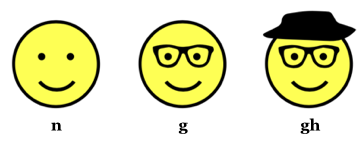
\includegraphics[width=.5\textwidth]{plots/faces-ad-hoc-implicature.png}
\caption{\label{fig:faces-ad-hoc-imp}: Referents in ad-hoc implicature reference game.}
\end{figure}

At the next level, pragmatic listeners $L_1$ try to infer the world state that the speaker intended to communicate
through Bayesian inference: $L_1$ integrates their prior beliefs about the state of the world $P(w)$ with the likelihood
of the speaker $S_1$ choosing the observed utterance to communicate $w$:
$$L_1(w \mid u) \propto P(w) \times S_1(u \mid w)$$

This recursive reasoning process can theoretically be continued ad infinitum by adding additional speaker and listener agents that 
reason about their respective counterpart agents one level below $i-1$ the current level $i$:
$$U_i(w,u) = \log L_{i}(w \mid u) - c(u)$$
$$S_i \propto \mbox{exp} \left( \lambda U_{i-1}(w,u) \right)$$
$$ L_i(u \mid w) \propto P(w) \times S_i(u \mid w)$$

\todo{mention IBR}

In practice, however, this recursive process is usually capped at the $L_1$ and $L_2$ level (\todo{add reference. Franke and Degen?}) and the models
that I will consider in this dissertation are also all capped at the $L_1$ level.



This recursive reasoning process implicitly models a Gricean counterfactual reasoning process in which listeners reason about alternative utterances
that a speaker could have produced but didn't to interrpret To illustrate how this works, consider a simple reference game as shown in Figure~\ref{fig:faces-ad-hoc-imp}.\footnote{Example adapted from \cite{GoodmanFrank2016}.} In this game,
there are three faces: one without any accessories (\textbf{n}), one with glasses (\textbf{g}), and one with glasses and a hat (\textbf{gh}). A speaker chooses one of the three faces
and tries to communicate her choice to the listener through an utterance $u$. In this contrived example, let us assume that the only three possible utterances that the
speaker can choose from are $U=\{\mbox{\textsc{face}: My friend has a face},\mbox{\textsc{glasses}: My friend has glasses},$ $\mbox{\textsc{hat}: My friend has a hat}\}$, 
and that the listener is aware that the speaker can only choose from these three utterances. Speakers tend to show the following behavior in this game. If they refer
to \textbf{n}, they produce \textsc{face}, if they refer to \textbf{g}  they produce \textsc{glasses}, and if they refer to \textbf{gh} they produce \textsc{hat}. Conversely, listeners infer that 
the speaker likely referred to \textbf{n} after hearing \textsc{face}, to \textbf{g}  after hearing \textsc{glasses}, and to \textbf{gh} after hearing \textsc{hat}.

An RSA model rooted at a literal listener $L_0$ with a pragmatic speaker $S_1$ and a pragmatic listener $L_1$ captures this behavior. In this game, 
the semantic interpretation function $\sem{\cdot}$ is defined as:

\begin{center}
\begin{tabular}{c | c } 
$u$ & \sem{u} \\ \midrule
\textsc{face} & $\{\mathbf{n}, \mathbf{g} , \mathbf{gh}\}$  \\
\textsc{glasses} & $\{ \mathbf{g} , \mathbf{gh}\}$ \\
\textsc{hat} &$\{\mathbf{gh}\}$ \\
\end{tabular}
\end{center}

\noindent Computing the distributions for $L_0 (w\mid u)$ -- if we assume uniform priors over the three referents -- then results in:

\begin{center}
\begin{tabular}{c | c | c | c} 
$u$ & $L_0( \mathbf{n} \mid u)$ &  $L_0( \mathbf{g} \mid u)$ &  $L_0( \mathbf{gh} \mid u)$ \\ \midrule
\textsc{face} & $\frac{1}{3}$ & $\frac{1}{3}$ & $\frac{1}{3}$  \\
\textsc{glasses} &0  & $\frac{1}{2}$ & $\frac{1}{2}$  \\
\textsc{hat} & 0 & 0 & 1 \\
\end{tabular}
\end{center}

\noindent At the two extremes, $L_0$ thus chooses a face at random after hearing \textsc{face}, which is true about all three 
faces but it will always choose \textbf{gh} after hearing \textsc{hat}, which is only true for \textbf{gh}. As I mentioned above, the
pragmatic speaker $S_1$ then chooses an utterance by soft-maximizing their utility, which depends on the informativity of $u$
to communicate $w$ to $L_0$ and the cost $c(u)$, which I assume to be 0 for all utterances in this example. If we further assume
that the rationality parameter $\lambda=1$, then $S_1(u \mid w)$ is:

\begin{center}
\begin{tabular}{c | c | c | c} 
$w$ & $S_1( \textsc{face} \mid w)$ &  $S_1( \textsc{glasses} \mid w)$ &  $S_1( \textsc{hat} \mid w)$ \\ \midrule
\textbf{n} & 1  & 0 & 0  \\
\textbf{g} &$\frac{2}{5}$  & $\frac{3}{5}$ & 0  \\
\textbf{gh} & $\frac{2}{11}$ & $\frac{3}{11}$ & $\frac{6}{11}$ \\
\end{tabular}
\end{center}

\noindent This speaker model qualitatively predicts the behavioral data from forced choice production experiments \cite{GoodmanFrank2016}: for all three
referents the most likely utterance choice according to $S_1$ matches the most likely choice in the experimental data. However, this behavior could have
also been predicted by purely symbolic counterfactual reasoning processes as outlined in \cite{Grice1975, Hirschberg1989}. The real advantage of this model 
comes from the fact that it is a quantitative model and if one fits the rationality parameter $\lambda$ to the experimental data, one can also quantitatively predict 
utterance choices in a population of participants.

Finally, the pragmatic listener $L_1(w \mid u)$ can be used to predict the interpretation of utterances in this context. If we again assume that the prior over referents $P(w)$
is uniform, $L_1$ is:

\begin{center}
\begin{tabular}{c | c | c | c} 
$u$ & $L_1( \mathbf{n} \mid u)$ &  $L_1( \mathbf{g} \mid u)$ &  $L_1( \mathbf{gh} \mid u)$ \\ \midrule
\textsc{face} & $\frac{55}{87}$ & $\frac{22}{87}$ & $\frac{10}{87}$  \\
\textsc{glasses} &0  & $\frac{11}{16}$ & $\frac{5}{16}$  \\
\textsc{hat} & 0 & 0 & 1 \\
\end{tabular}
\end{center}

\noindent This listener model qualitatively predicts the behavioral data from the interpretation experiments, and once again one can quantitatively predict participants' proportions
of choosing the three referents after hearing a given utterance by fitting the rationality parameter $\lambda$. 

Predicting utterance choices and interpretations in this contrived example of an ad-hoc implicature may not seem particularly impressive. However, many subsequent works
following the original RSA model have extended this basic model to predict a wide range of pragmatic phenomena, including predicting scalar inferences 
\cite{GoodmanStuhlmuehller2013}, embedded implicatures \cite{Potts2016}, M-implicatures \cite{Bergen2016}, metaphors and hyperbole \cite{Kao2013,Kao2014,Kao2015}, 
irony \cite{Kao,CohnGordon2019}, the use of gradable adjectives \cite{LassiterGoddman2015, QingFranke2014}, generics \cite{Tessler2019}, vague quantifiers 
\cite{SchoellerFranke2017}, politeness \cite{Yoon2019}, social meaning\cite{Burnett2017}, and -- as I will discuss in more detail in the next chapter -- 
to predict the use and interpretations of epistemic modals \cite{HerbstrittFranke2019}. While almost all of these models 
introduce additional extensions to the model as presented here, they crucially all rely on the recursive Bayesian reasoning process outlined in this section,
highlighting the versatility of models that cast pragmatic behavior as an instance of Bayesian reasoning.





